%!TEX program = lualatex
\documentclass{beamer}
\mode<presentation> {
    \usetheme{Marburg}
}
\usepackage[english]{babel}
\usepackage[style=english]{csquotes}
\usepackage{fontspec}
\usepackage{csquotes}
\usepackage{amsmath}
\usepackage{float}
\usepackage{graphicx} % Allows including images
\usepackage{booktabs} % Allows the use of \toprule, \midrule and \bottomrule in tables
\usepackage{makecell}
\usepackage{hyperref}
\usepackage{listings}
\usepackage{caption}
\captionsetup{font=scriptsize}
% TikZ configuration
\usepackage{tikz}
\usetikzlibrary{
    arrows,
    shapes
    % positioning,
    % shadows,
    % trees,
    % calc
}

% Define TikZ elements and styles
\tikzstyle{block} = [rectangle, draw, fill=blue!20,
    text centered, rounded corners, minimum height=2em]
\tikzstyle{line} = [draw, -latex']
\tikzstyle{cloud} = [draw, ellipse,fill=red!20, node distance=3cm,
    minimum height=2em]
\tikzset{
    plain/.style = {
        draw=none,
        fill=none
    }
}

% Biber configuration
\usepackage[
backend=biber,
style=alphabetic,
citestyle=authoryear,
natbib
]{biblatex}
\addbibresource{L0.bib}

% Configure section slides insertion
\AtBeginSection[]{
  \begin{frame}
  \vfill
  \centering
  \begin{beamercolorbox}[sep=8pt,center,shadow=true,rounded=true]{title}
    \usebeamerfont{title}\insertsection\par%
  \end{beamercolorbox}
  \vfill
  \end{frame}
}


\title[Introduction \& syllabus]{
    Introduction \& syllabus \\
    \small{}
}
\author{Szymon Talaga and Mikołaj Biesaga} % Your name
\institute[ISS UW]{
    The Robert Zajonc Institute for Social Studies \\ University of Warsaw \\
    \medskip
    \textit{stalaga@uw.edu.pl} \\
    \textit{m.biesaga@uw.edu.pl}
}
\date{\today} % Date, can be changed to a custom date


%%%%%%%%%%%%%%%%%%%%%%%%%%%%%%%%%%%%%%%%%%%%%%%%%%%%%%%%%%%%%%%%%%%%%%%%%%%%%%%

\begin{document}


%%% SLIDES %%%%%%%%%%%%%%%%%%%%%%%%%%%%%%%%%%%%%%%%%%%%%%%%%%%%%%%%%%%%%%%%%%%%
\frame{\titlepage}

\section{Introduction}


\begin{frame}[fragile]
    \frametitle{An Algorithm For Finding Primes Numbers.}
  \begin{semiverbatim}
  \uncover<1->{\alert<0>{int main (void)}}
  \uncover<1->{\alert<0>{\{}}
  \uncover<1->{\alert<1>{  \alert<4>{std::}vector<bool> is_prime (100, true);}}
  \uncover<1->{\alert<1>{  for (int i = 2; i < 100; i++)}}





\begin{frame}{What is computational social science?}
\begin{itemize}
    \item In the most general sense computational social science (CSS)
    is about addressing social-scientific problems with computational methods.
    \item It is closely related to the field of data science, which can be
    defined as set of theory \& practices related to answering research questions
    based on empirical data, including large volumes of unstructured numeric
    and textual data, using the scientific methods, processes and algorithms.
    It sits at the intersection statistics, computer science and mathematics.
\end{itemize}
\end{frame}

\begin{frame}{General interest in data science}
    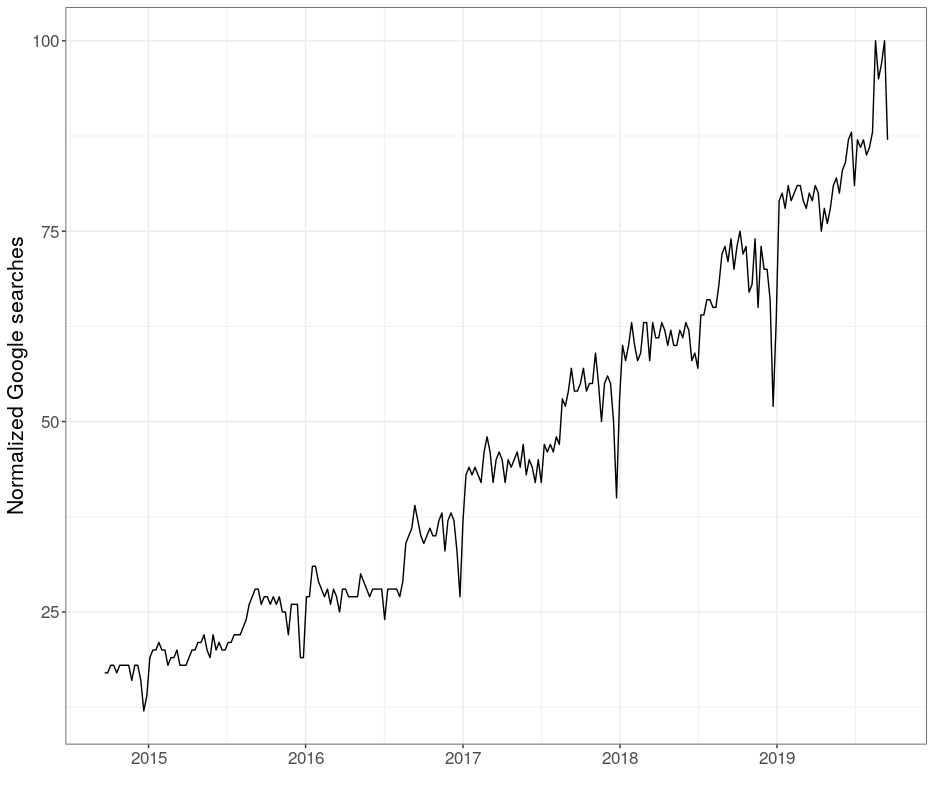
\includegraphics[width=\framewidth]{ds-searches.png}
\end{frame}

\begin{frame}{Computational methods\footnotetext{
    In this class we focuse on the parts written in bold.
}}
\begin{itemize}
    \item \textbf{Extraction of unstructured data from external digital (i.e. web-based)
    sources.}
    \begin{itemize}
        \item \textbf{Webscraping (extraction of data from existing webpages).}
        \item \textbf{Extracting data from web APIs (i.e. Twitter).}
    \end{itemize}
    \item \textbf{Analysis of textual data (natural language processing - NLP).}
    \item Network and relational data analysis.
    \item Working with big datasets (that do not fit into RAM of a single computer).
    In-database computations, distributed computing etc.
    \item Computer simulations.
    \item Online experiments (A/B testing, experiments based on online games etc.).
\end{itemize}
\end{frame}

\begin{frame}[fragile]{Data formats}
\begin{itemize}
    \item Computational studies often entail working with datasets that
    can not be easily represented with traditional data tables typically
    used in psychology and social sciences
    (respondents in rows, variables in columns).
    \item Usually one has to work with complicated semi-structured nested
    data formats like JSON:
    \begin{small}
    \begin{verbatim}
    { persons: [
        { name: "Alice", age: 17, interests: [
            { name: "sport", score: 7, tags: [
                "physical activity",
                "outdoor"
            ] }
        ] },
        { name: "Bob", age: 18, interests: [] }
    ] }
    \end{verbatim}
    \end{small}
\end{itemize}
\end{frame}

\begin{frame}{Goal of the class}
\begin{itemize}
    \item In general the practice of data science and computational social science
    requires a lot of technical skills such as computer programming and statistics,
    which can not be taught in a brief one-semester course like this.
    \item However, not everyone in a research project has to be a techie.
    \item But it is necessary that everyone in a team has the basic knowledge
    about modern computational technologies and methods, so everyone shares
    the same language which makes it possible to communicate efficiently regardless
    of difference in background and training.
    \item This class is meant to teach you this language, so you can
    collaborate with technical persons and design computationally-oriented
    studies.
\end{itemize}
\end{frame}


\section{Syllabus \& rules}

\begin{frame}{Syllabus}
\begin{itemize}
    \item All the rules as well as the outline of the class are described in
    detail in the syllabus. It can be accessed via our Google drive and Slack
    workspace\footnotetext{
        \tiny{\href{https://drive.google.com/a/uw.edu.pl/file/d/1VotLZIEmp4lXnT-NdR0yZ5DDal59FfkI/view?usp=sharing}{https://drive.google.com/a/uw.edu.pl/file/d/1VotLZIEmp4lXnT-NdR0yZ5DDal59FfkI/view?usp=sharing}}
    }.
\end{itemize}
\bigskip

\includegraphics[width=\framewidth]{syllabus.png}
\end{frame}

\begin{frame}{General advice}
\begin{itemize}
    \item In this class we do not expect any background in computer science,
    programming etc.
    \item However, it will be relatively difficult, especially for those of you
    who are not particularly tech-savvy.
    \item This is why it is absolutely crucial to try to do all the homework
    we will assign to you, as they are necessary for you to internalize
    the material.
    \item You are allowed to miss up to two classes. However, we really recommend
    to attend all of them, as some parts of the material will build on the
    earlier parts.
\end{itemize}
\end{frame}

\begin{frame}{Assessment criteria}
\begin{itemize}
    \item There are three assessment components:
    \begin{enumerate}
        \item 3 homework assignments.
        \item Final exam.
        \item Written research project. You will have to write a research proposal
        for a project using some of the computational methods we will cover
        in the class.
    \end{enumerate}
    \item Final grade = 30\%$\times$homeworks + 35\%$\times$final exam +
    35\%$\times$written report
    \item Grading scale\footnotetext{
        Non-integer percentages will be always rounded upwards.
    }:
    \begin{itemize}
        \item 5 --- 90-100\% (outstanding performance)
        \item 4+ --- 85-89\%
        \item 4 --- 75-84\% (good performance)
        \item 3+ --- 70-74\%
        \item 3 --- 60-69\% (minimum passing performance)
        \item 2 -- 59\% or less (fail)
    \end{itemize}
\end{itemize}
\end{frame}

%%% LITERATURE %%%%%%%%%%%%%%%%%%%%%%%%%%%%%%%%%%%%%%%%%%%%%%%%%%%%%%%%%%%%%%%%
\begin{frame}{Literature to read}
\nocite{*}
\AtNextBibliography{\footnotesize}
\printbibliography
\end{frame}

\begin{frame}{Closing remarks}
    \begin{itemize}
        \item This is the first edition of this course.
        \item Feel free to let us know when something does not work well for you.
    \end{itemize}
    \end{frame}


%%%%%%%%%%%%%%%%%%%%%%%%%%%%%%%%%%%%%%%%%%%%%%%%%%%%%%%%%%%%%%%%%%%%%%%%%%%%%%%

\end{document}
